\documentclass[10pt,border=3pt]{standalone}
\usepackage{amsmath,amssymb,bm}
\usepackage{tikz}
\usetikzlibrary{arrows.meta,calc,positioning,backgrounds,fit}
\begin{document}
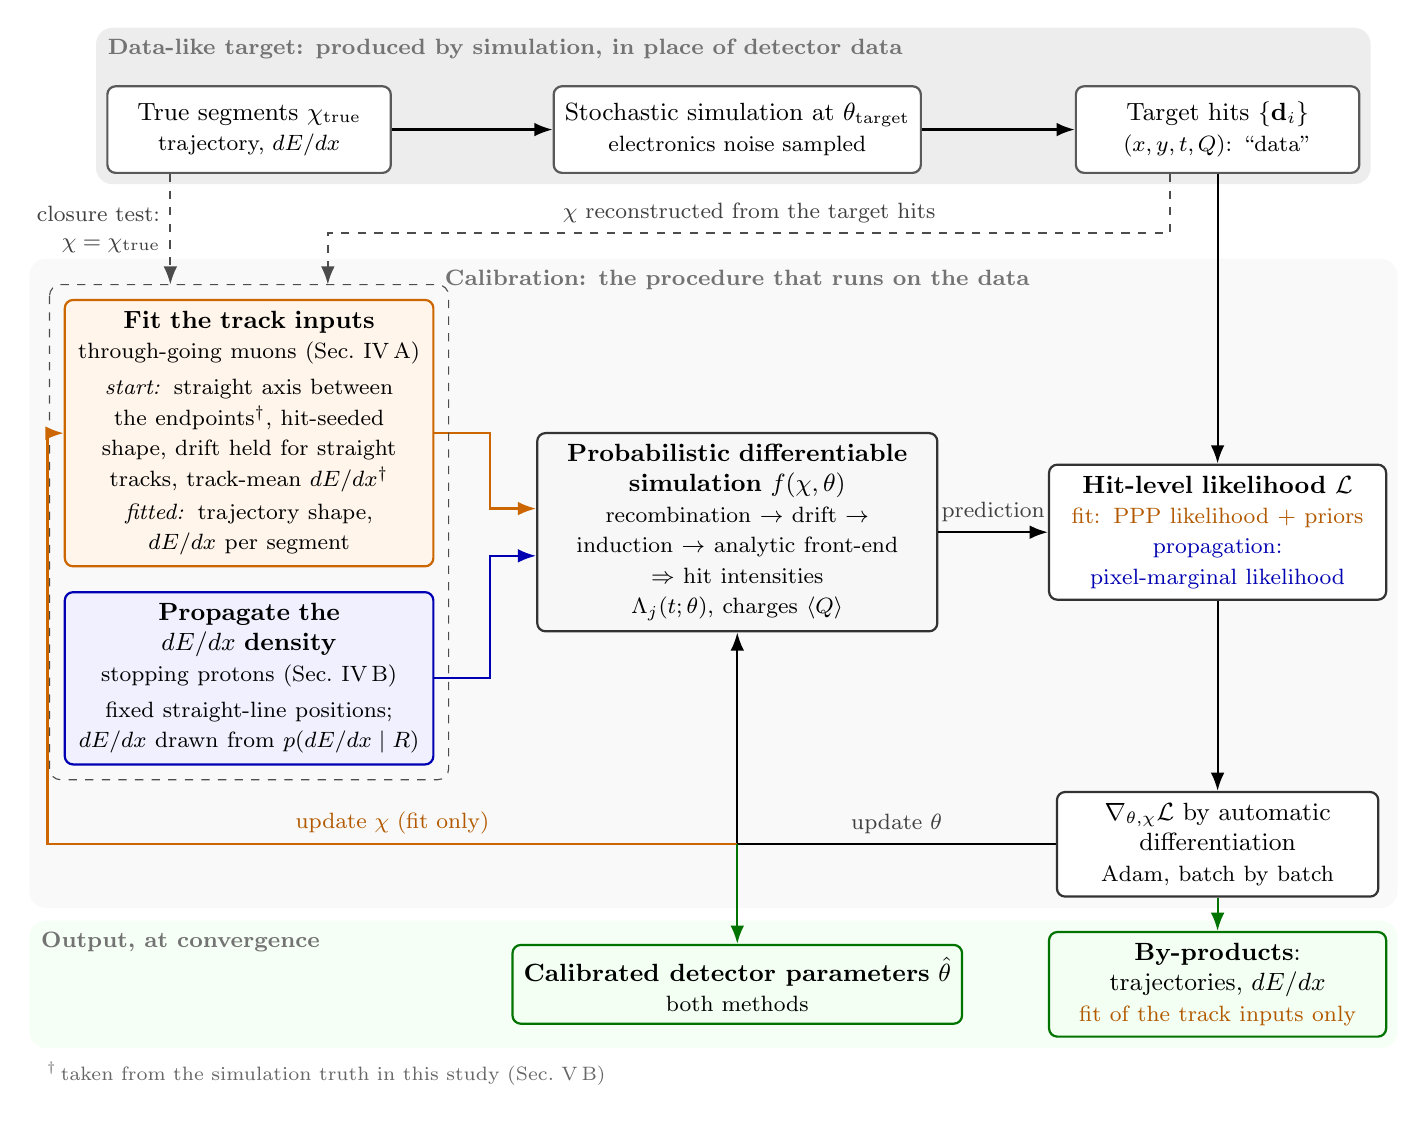
\begin{tikzpicture}[
    >=Latex,
    font=\small,
    box/.style={draw, rounded corners=3pt, thick, align=center, inner sep=4pt, fill=white, execute at begin node={\hyphenpenalty=10000\exhyphenpenalty=10000}},
    tgt/.style={box, draw=gray!70!black},
    sim/.style={box, draw=black!80, fill=black!3},
    mu/.style={box, draw=orange!80!black, fill=orange!8},
    pr/.style={box, draw=blue!70!black, fill=blue!6},
    outb/.style={box, draw=green!45!black, fill=green!5},
    lbl/.style={font=\footnotesize, align=center, text=black!75},
    band/.style={rounded corners=6pt, draw=none, inner sep=1.3mm},
    bandlbl/.style={font=\footnotesize\bfseries, text=black!55, anchor=north west, inner sep=1.5mm},
    flow/.style={->, thick},
    dflow/.style={->, thick, dashed},
]
    % ---------------- Row 1: data-like target ----------------
    \node[tgt, minimum width=36mm, minimum height=11mm] (truth) at (0,0)
        {True segments $\chi_{\rm true}$\\{\footnotesize trajectory, $dE/dx$}};
    \node[tgt, minimum width=46mm, minimum height=11mm] (stoch) at (6.2,0)
        {Stochastic simulation at $\theta_{\rm target}$\\{\footnotesize electronics noise sampled}};
    \node[tgt, minimum width=36mm, minimum height=11mm] (data) at (12.3,0)
        {Target hits $\{\mathbf d_i\}$\\{\footnotesize $(x,y,t,Q)$: ``data''}};
    \draw[flow] (truth) -- (stoch);
    \draw[flow] (stoch) -- (data);
    % ---------------- Row 2: inputs -> forward model -> loss ----------------
    \node[mu, minimum width=46mm, text width=44mm, anchor=north] (muin) at (0,-2.15)
        {\textbf{Fit the track inputs}\\{\footnotesize through-going muons (Sec.~IV\,A)}\\[2pt]
         {\footnotesize\textit{start:} straight axis between the endpoints$^\dagger$, hit-seeded shape, drift held for straight tracks, track-mean $dE/dx^\dagger$}\\[1pt]
         {\footnotesize\textit{fitted:} trajectory shape, $dE/dx$ per segment}};
    \node[pr, minimum width=46mm, text width=44mm, anchor=north] (prin) at ($(muin.south)+(0,-3mm)$)
        {\textbf{Propagate the $dE/dx$ density}\\{\footnotesize stopping protons (Sec.~IV\,B)}\\[2pt]
         {\footnotesize fixed straight-line positions; $dE/dx$ drawn from $p(dE/dx\mid R)$}};
    \coordinate (mid) at ($(muin.north)!0.5!(prin.south)$);
    \coordinate (xf) at (6.2,0); \coordinate (xl) at (12.3,0); \coordinate (xleft) at (-2.56,0);
    \node[sim, minimum width=50mm, text width=48mm, minimum height=16mm] (fwd) at (xf |- mid)
        {\textbf{Probabilistic differentiable simulation} $f(\chi,\theta)$\\{\footnotesize recombination $\to$ drift $\to$ induction $\to$ analytic front-end}\\{\footnotesize $\Rightarrow$ hit intensities $\Lambda_j(t;\theta)$, charges $\langle Q\rangle$}};
    \node[box, draw=black!80, minimum width=42mm, text width=40mm, minimum height=16mm] (loss) at (xl |- mid)
        {\textbf{Hit-level likelihood} $\mathcal L$\\{\footnotesize\color{orange!70!black} fit: PPP likelihood + priors}\\{\footnotesize\color{blue!70!black} propagation: pixel-marginal likelihood}};
    \draw[flow, orange!80!black] (muin.east) -- ++(7mm,0) |- ([yshift=3mm]fwd.west);
    \draw[flow, blue!70!black] (prin.east) -- ++(7mm,0) |- ([yshift=-3mm]fwd.west);
    \draw[flow] (fwd) -- node[above, lbl] {prediction} (loss);
    \draw[flow] (data) -- (loss);
    \draw[gray!60!black, dashed, rounded corners=4pt] ($(muin.north west)+(-1.8mm,1.8mm)$) rectangle ($(prin.south east)+(1.8mm,-1.8mm)$);
    \coordinate (frametop) at ($(muin.north)+(0,1.8mm)$);
    \draw[dflow, gray!60!black] ([xshift=-6mm]data.south) -- ++(0,-0.75) -| ([xshift=10mm]frametop)
        node[pos=0.25, above, lbl] {$\chi$ reconstructed from the target hits};
    \draw[dflow, gray!60!black] ([xshift=-10mm]truth.south) -- ([xshift=-10mm]frametop)
        node[midway, left, lbl, align=right] {closure test:\\$\chi=\chi_{\rm true}$};
    % ---------------- Row 3: gradient update loop ----------------
    \coordinate (row3) at ($(prin.south)+(0,-10mm)$);
    \node[box, draw=black!80, minimum width=40mm, text width=38mm] (upd) at (xl |- row3)
        {$\nabla_{\theta,\chi}\mathcal L$ by automatic differentiation\\{\footnotesize Adam, batch by batch}};
    \draw[flow] (loss) -- (upd);
    \draw[flow] (upd.west) -- (upd.west -| fwd.south) node[pos=0.5, above, lbl] {update $\theta$} -- (fwd.south);
    \draw[flow, orange!80!black] (upd.west -| fwd.south) -- (xleft |- upd.west) node[pos=0.5, above, lbl, text=orange!70!black] {update $\chi$ (fit only)} |- (muin.west);
    % ---------------- Row 4: outputs ----------------
    \coordinate (row4) at ($(upd.south)+(0,-11mm)$);
    \node[outb, minimum width=50mm, minimum height=10mm] (cal) at (xf |- row4)
        {\textbf{Calibrated detector parameters} $\hat\theta$\\{\footnotesize both methods}};
    \node[outb, minimum width=42mm, text width=40mm, minimum height=10mm] (byp) at (xl |- row4)
        {\textbf{By-products}: trajectories, $dE/dx$\\{\footnotesize\color{orange!70!black} fit of the track inputs only}};
    \draw[flow, green!45!black] (upd.south) -- (byp.north);
    \draw[flow, green!45!black] (upd.west -| fwd.south) -- (cal.north);
    % ---------------- bands ----------------
    \begin{scope}[on background layer]
        \node[band, fill=black!7, fit={(truth) (stoch) (data) ($(truth.north west)+(0,6mm)$)}] (b1) {};
        \node[band, fill=black!2.5, fit={($(xleft |- frametop)+(-1mm,2mm)$) (prin) (fwd) (loss) (upd) ($(xleft |- upd.south)$)}] (b2) {};
        \node[band, fill=green!4, fit={(cal) (byp) ($(xleft |- cal.north)+(-1mm,0)$)}] (b3) {};
    \end{scope}
    \node[bandlbl] at (b1.north west) {Data-like target: produced by simulation, in place of detector data};
    \node[bandlbl, anchor=north] at (xf |- b2.north) {Calibration: the procedure that runs on the data};
    \node[bandlbl] at (b3.north west) {Output, at convergence};
    \node[font=\scriptsize, text=black!60, anchor=north west] at ($(b3.south west)+(1mm,-0.5mm)$) {$^\dagger$\,taken from the simulation truth in this study (Sec.~V\,B)};
\end{tikzpicture}
\end{document}
